\documentclass[12pt,a4paper]{report}

\usepackage{graphics}
\usepackage{fullpage,epsf,graphicx}
\usepackage{amsmath}%, amstext,url}
\usepackage{comment}
\usepackage{hyperref}
\usepackage{verbatim}
\usepackage{float}
\usepackage{placeins}
\usepackage{subcaption}
\graphicspath{{figures/}}
\def\BibTeX{{\rm B\kern-.05em{\sc i\kern-.025em b}\kern-.08em
    T\kern-.1667em\lower.7ex\hbox{E}\kern-.125emX}}

\begin{document}

\thispagestyle{empty}

%
%	This is a basic LaTeX Template for the TP/MP MSc Dissertation report

\parindent=0pt          %  Switch off indent of paragraphs 
\parskip=5pt            %  Put 5pt between each paragraph  

%	This section generates a title page
%       Edit only the sections indicated to put in the project title, and submission date

\vspace*{0.1\textheight}

\begin{center}
        \huge{\bfseries Event Attribution}\\ % Replace with the title of your dissertation!
\end{center}

\medskip

\begin{center}
        \Large{Christopher Long}\\  % Author of dissertation - replace with your name!
        \medskip
        \large{August 18, 2023}  % Submission date
\end{center}

%%% If necessary, reduce the number 0.4 below so the University Crest
%%% and the words below it fit on the page.
%%% Don't let the crest, or the wording below it, flow onto the next page!

\vspace*{0.4\textheight}

\begin{center}
        
\includegraphics[width=35mm]{crest}
\end{center}

\medskip

\begin{center}

\large{
  MSc in Mathematical Physics\\[0.8ex]
  The University of Edinburgh\\[0.8ex]
  2023}

\end{center}

\newpage


\pagenumbering{roman}

\begin{abstract}

Extreme rainfall on 12 August 2020 caused the Stonehaven Derailment,
    which resulted in three deaths.
This project applies current event attribution techniques for extreme rainfall events,
    finding a probability ratios for the extreme rainfall to be 1.1, 1.3 and 1.6 for the 1980s, 2010s and in a 2K warmer world
    respectively over pre-industrial.

\end{abstract}

\pagenumbering{roman}

\begin{center}
\textbf{Declaration}
\end{center}

I declare that this report is entirely my own work unless stated otherwise.

The introduction, chapter~\ref{ch:intro}, describes the motivations for the work.
This includes the information showing the impact of the extreme rainfall on the derailment by the Rail Accident Investigation Board~\cite{RAIB_2022},
    as well as my supervisor's paper analysing the effect of climate change on the risk of an extreme rainfall event~\cite{Tett_Soon}.

Chapter~\ref{ch:attribution} contains background material,
    with the first and third sections primarily relying on World Weather Attribution's methodology~\cite{van_Oldenborgh_et_al_2021},
    and the second section makes use of the information in Coles' textbook on the topic~\cite{Coles_2001}.

Chapter~\ref{ch:dev} consists of my own work,
    excepting the use of code and creation of equivalent diagrams to a currently approved but not yet published paper by my supervisor.
Code used in this project is given in~\cite{Me_Code},
    code used in my supervisor's paper is given in~\cite{Tett_Code}

Chapter~\ref{ch:results} is entirely my own work.

\bigskip

Calculations used Python with many standard packages.

NumPy and XArray are used to manage and process both real and modelled rainfall data.

CartoPy is used to process data between both Ordinance Survey and Longitude-Latitude coordinate systems.

R and the RPy package are used to fit extreme value distributions to the rainfall data.
This calls the extRemes R package~\cite{extremes_R}.

The Rain Radar Data is taken from the Met Office's NIMROD system~\cite{radar_data}.

The Model Data is taken from the Met Office Hadley Centre's UKCP18 Convection-Permitting Model projections~\cite{model_data}.

Tht topography data on an OSGB grid is taken from~\cite{radar_topog}.

The data processing ran on both the JASMIN supercomputer and on my local machine,
GitHub was used to manage the transfer of both code and data.

The majority of the code used in this project is based on the code used by my supervisor performing a similar analysis on the 2021 Edinburgh cloudburst~\cite{Tett_Soon}.


\newpage

\begin{center}
\textbf{Personal Statement} % Use Git commits
\end{center}

I spent the first 2 weeks of the project retro-fitting the Edinburgh castle
library to apply to the Stonehaven crash.
This process began by creating plots including the
rainfall at the crash location on the day and an animation of the rainfall
in the Stonehaven region, allowing me to find an appropriate event definition.

For the remaining weeks of June, I implemented a topographical height mask
to the radar data, as well as establish a workspace to transfer data between
my laptop and the JASMIN supercomputer.

Following this I began my analysis of the radar data.
This involved computing and plotting the monthly rainfall maxima in
the Stonehaven region, as well as finding the quantiles of these extrema,
as well as using R to find the parameters of a GEV fit to both the empirical
and a monte carlo bootstrap of the rainfall distribution.

In mid-July, I created plots for these distributions and started to work with the Convection Permitting Model data,
    processing it as necessary to be appropriate for the use case.
This allowed me to create the time series to act as covariates to the CPM rainfall data,
    which were used in the first week of August to compute the probability ratios, intensity ratios and plots.
Any work done in August other than writing up the dissertation was spent analysing and critiquing the techniques used.

I started writing this dissertation in mid-July, and I spent the first
three weeks of August working on it full-time.

I have achieved the final outcome of probability ratios for the event and
    discussed the limitations of these results.


\newpage

\begin{center}
%\vspace*{2in}
% an acknowledgements section is completely optional but if you decide
% not to include it you should still include an empty {titlepage}
% environment as this initialises things like section and page numbering.
\textbf{Acknowledgements}
\end{center}

I'd like to thank my supervisor Professor Simon Tett for
making this project possible.



\tableofcontents
\listoftables
\listoffigures

\pagenumbering{arabic}

\chapter{Introduction}\label{ch:intro}

\section{Stonehaven Derailment}\label{sec:stonederail}

%  TODO use RAIB analysis

\section{Rainfall in a warmer world}\label{sec:warmerrainfall}

%  TODO rely on Simon's paper and other references
\begin{comment}
The Introduction should contain a description of your project and the
problem you are trying to solve. It should start off at a level that
should be understandable by anyone with a degree in physics, but it
can become more technical later

Where appropriate you should include references to work that has
already been done on your topic and anything else which lets you set
your work in context.
\end{comment}

\chapter{Event Attribution Theory}\label{ch:attribution}

As a part of a complex system,
    any weather event is necessarily multifactorial,
    with no single cause.
It is therefore necessary to use a probabilistic lens to perform a scientific analysis.

In this case, the weather at a given place and time of year is expressed as a statistical distribution of events.
The climate may then be considered either the distribution itself,
    or the parameters informing the distribution.
In other words, ``Climate is what we expect, weather is what we get.''~\cite{Herbertson_1935}.

The scientific method may then be applied,
    using the climate distribution as a dependent variable to the factor being considered.
Issues, of both a technical and a theoretical nature can arise with this approach,
    and will be discussed in subsection~\ref{sec:attrchallenge}.

In all the examples given in this section,
    the independent variable is anthropogenic climate change.
This is often quantified by using a temperature metric,
    although additional factors may be considered.

It may be noted that,
    due to their generality,
    climate event attribution techniques may be of use outside risk analysis from modern changes in the climate.
For example,
    Ruddiman~\cite{Ruddiman_2010} has attempted to attribute the lack of a recent glaciation to the beginning of agriculture.

An event attribution study aims to provide two quantities.
The first is the change in the probability of the event.
The second is the change in the magnitude of the event.

\subsubsection{Development of Event Attribution}

In 2003, whilst experiencing flooding as a result of extreme weather,
    Allen~\cite{Allen_2003} posited the probabilistic interpretation of climate change impacts,
    proposing a potential to find greenhouse gas emitters liable for extreme weather events.
%  Add note about the fact that a grant would not be paid to emitters for reducing the likelihood.
A notable early use case of this probabilistic approach was by Stott et al.~\cite{Stott_2004},
    finding that 75\% of the risk of the European heatwave is attributable to anthropogenic climate change.

World Weather Attribution produces rapid Event Attribution studies,
    some of which are within a month of the event occuring~\cite{van_Oldenborgh_et_al_2018},
    using the probabilistic approach.
Alternative approaches also exist.
One of these is the `Boulder' methodology,
    described in section 2.2 of~\cite{Otto_2017},
    which seeks to break down the proportions to which the event was caused by natural variability and the due to Anthropogenic Climate Change.
Another is the `storyline' methodology,
    outlined by Shepherd et al.\ in~\cite{Shepherd_et_al_2018},
    although this has been considered contentious~\cite{García-Portela_Maraun_2023}.

\section{Steps to Event Attribution}\label{sec:attrsteps}

The precise number of steps for successful event attribution vary by the situation.
Van Oldenborgh et al.~\cite{van_Oldenborgh_et_al_2021} give 8 separate steps,
    while Otto~\cite{Otto_2017} gives 6 steps.
Both of these methodologies are functionally identical;
    I shall base my description upon 4 of the steps described by Otto.

Only four steps are given in full below.
This is due to the removal of an analysis trigger step at the start of the process
    and a communication step at the end of the process,
    both of which I will cover here briefly.

An analysis trigger is a set of criteria used to determine whether an event should be investigated.
These serve a utilitarian purpose,
    allowing the events with the greatest impact to be investigated first.
These may include the number of deaths or number impacted,
    as in chapter 2 of~\cite{van_Oldenborgh_et_al_2021},
    or economic and cultural factors, as in~\cite{Tett_Soon}.
The former criteria may skew analysis towards poorer nations~\cite{Kahn_2005},
    while the latter may skew analysis towards richer nations.

It is of note that potential liability of anthropogenic climate change may be a triggering factor,
    so the analysis begins due to a hypothesis that the event was caused by anthropogenic climate change.
I believe that this may bias the results of a meta-analysis of event attribution studies,
    and so increase the challenge in determining anthropogenic climate change as a cause of more extreme events in general.
I omit giving any further detail on the analysis trigger as it is beyond the scope of mathematical or physical interest.

The communication of the outcome of the analysis may also be considered in the study.
This is especially true outside the scientific community
    and considers the risk of the audience drawing incorrect conclusions,
    as well as the risk of policymakers acting on incorrect information.

\subsection{Event Definition}\label{subsec:backeventdef}

To perform an attribution analysis,
    the weather event must first be defined in clear and quantitative terms.
This requires specifying a variable with a threshold that has been crossed,
    as well as the time and region at which an event may be considered.

This is not necessarily straightforward.
An event attribution is normally triggered by the event's social or environmental impact,
     not just due to the meteorological significance.
Therefore, care must be taken to ensure that the definition of the event is sufficiently similar to the conditions that would cause a similar impact.

Many of the challenges in Event Attribution arise directly from a poor Event Definition.
Events that are too narrowly defined may have issues with reproducibility,
    as will be discussed in~\ref{subsec:eventrepro},
    while events that are too widely defined may give invalid results,
    as will be discussed in~\ref{subsec:modelvalid}.

\subsubsection{Variable and Threshold}

The climate variable used to define the event requires travelling up the causal chain that leads to it.
As a set of examples,
    floods/droughts are caused by extreme highs/lows in rainfall,
    while heat waves and cold spells are caused by extreme high or low temperatures.

However,
    all of these events require the extreme rainfall/temperature to be sustained for the event to be hazardous.
Simple metrics may be applicable here,
    as the definition can then use the rainfall/temperature averaged over a given time period.
The selection of time period itself also requires a consideration of the event.
A damaging heavy storm requires extreme winds over a matter of minutes,
    while it may take days for the land to dry out sufficiently for a drought to occur.

More advanced metrics may be used.
For example, an Expert Team on Climate Change Detection Indices~\cite{Zhang_2011}
    describes a `Growing Season Length',
    allowing climate-caused famine to be quantified using only daily temperature data.
A `Wet-Bulb Temperature' has been used to combine humidity and temperature data to create an index that better measures teh effect of a heatwave on human health~\cite{Li_2020}.

\subsubsection{Spatial and Temporal Region}

In addition to defining a threshold variable,
    it is necessary to define the regions and times at which an event can be considered sufficiently similar to that being analysed.
This is due to the fact that both historical trend analysis is impossible on a single extreme event at a single place on a single day of the year
    and that climate models will rarely reproduce events in such a narrow definition.
The second of these factors will be discussed in subsection~\ref{subsec:eventrepro}.

For the spatial region,
    a region with a known climate similar to that in which the event occurred is chosen,
    typically directly around the location of the event.
This is done so that the frequency and types of event will match the location of the original event,
    as well as to ensure that the factors that change the climate,
    whether Anthropomorphic or not,
    are similar to those changing the climate at the point of the event.

In addition to the aforementioned similarity in location,
    a historical trend analysis can aid in defining a region,
    along with tools including topography and climate classifications.
The region is chosen based on similar weather,
    not a similarity in hazard risk,
    as the goal is to perform an attribution for the event,
    not to advise on potential future risk.
For example,
    a region defined for a flood event over a flood-prone area would only consider areas with similar rainfall,
    not those similarly flood-prone.

For the temporal region,
    or time period for the event to be considered,
    an analogous process must be used.
It is often appropriate to use a seasonal time period,
    as this can also limit the event to those with similar meteorology,
    such as by only considering monsoon rainfall~\cite{Otto_et_al_2023}.
This can also prove to be a practical step,
    reducing the amount of data to be used later in the attribution process.

Additional `Boundary Conditions'~\cite{van_Oldenborgh_et_al_2021} may then also be imposed.
Of note is the importance of the El Niño,
    especially for drought events in the southern hemisphere~\cite{Lyon_2004},
    so this may also be accounted for when defining these event.

Once all of these definitions have been made,
    a `class' of events has been described.
This class will then be used to find like events in both the historical and model data.

\subsection{Model Evaluation}\label{subsec:backmodeleval}

\subsection{Likelihood Estimation}\label{subsec:backlikeest}

\subsection{Interpretation}\label{subsec:backinterp}

\section{Extreme Value Statistics}\label{sec:exstats}

This subsection will describe the statistical foundations of extreme event modelling,
    paraphrasing Coles' book~\cite{Coles_2001} unless where otherwise stated.
Climate events that pose hazards are necessarily extreme.
Therefore, to model these events,
    extreme value distributions are necessary.

Throughout the analysis,
    we assume that the variables are independent and identically distributed ($i.i.d.$).
The issues that may arise from this assumption not being valid are considered in subsection~\ref{subsec:statvalid}.

For event definitions which average a variable over a season,
    as opposed to focusing on the extreme
    a normal distribution is instead appropriate.
This is as the Central Limit Theorem states that the limit of the mean of $n$ $i.i.d.$ random variables tends to a normal distribution.
The equivalents for extreme events, the GEV distribution and Extremal Types Theorem,
    will be explained in due course.

\subsection{GEV Distribution}\label{subsec:gev}

\subsubsection{Extremal Types Theorem}

This explanation is as given in section 3.1 of~\cite{Coles_2001}.

Let $M_n$ be the maximum of $n$ $i.i.d.$ random variables.
If there exist sequences of constants $a_n > 0$ and $b_n$, and non-degenerate $G$ such that:

\[ P\left( \frac{M_n - b_n}{a_n}  \leq z \right) \rightarrow G(z) \text{ as } n \rightarrow \infty \]

Then $G$ is a member of the GEV (Generalised Extreme Value) family.

Section 3.1.4  of~\cite{Coles_2001} outlines a proof of the Extremal Types Theorem.
This involves showing that being a GEV distribution is equivalent to being `Max-Stable',
    then that the maxima of GEV distributions are Max-Stable,
    giving the GEV as the distribution of the original maximum in the infinite limit.
It is of note that this is similar to one approach to proving the Central Limit Theorem,
    which considers the normal distribution as a unique fixed point under convolutions,
    resulting in normal distributions being an infinite limit of the sum or mean~\cite{Hamedani_Walter_1984}.

Section 3.5 of~\cite{Coles_2001} shows, \textit{mutatis mutandis},
    that the extremal types theorem applies identically to minima by reversing the sign of the data.

\subsubsection{Parameters and Types of GEV distributions}

The GEV distribution has a CDF given by:
\begin{equation}\label{eq:gevcdf}
    G(z) = \exp \left( - \left( 1 + \xi \left( \frac{z-\mu}{\sigma} \right)  \right)^{-\frac{1}{\xi}} \right)
\end{equation}

This has three parameters, the location $\mu$, the scale $\sigma$ and the shape $\xi$.
It is clear from this CDF that the change of location and scale parameters represent moving and rescaling the distribution,
    much as the mean and standard deviation parameters do for a normal distribution.

The shape parameter determines the thickness of the tail of the distribution.
The larger the shape parameter, the thicker the tail of the distribution.

%  TODO insert graph w different shape parameters

Where $\xi > 0$,
    the distribution is heavy-tailed.
This type of GEV distribution is also known as a Fr\'{e}chet distribution.
Special cases of this distribution have unique properties,
    where $\xi \geq \frac{1}{2}$, the distribution has infinite variance and
    where $\xi \geq 1$, the distribution has infinite mean.

Where $\xi < 0$, the distribution is bounded,
    also known as a reversed Weibull distribution.
These distributions are limited to a maximum `most extreme' value of $\mu - \frac{\sigma}{\xi}$.
It can therefore be expected that distributions modelling extrema with physical constraints would have a negative shape parameter.
For example, Table 3 of Chikobvu and Chifurira's paper~\cite{Chikobvu_2015} modelling rainfall minima finds a negative shape parameter,
    which would be expected as rainfall cannot be negative.

Where $\xi = 0$,
    the distribution is a Gumbel distribution.
The CDF of this distribution requires taking the limit as $\xi \rightarrow 0$,
    giving a double exponential CDF\@.
The extrema of normal distributions converge to a Gumbel distribution,
    shown as a step in the proof of Proposition 1 of~\cite{Bailey_2014}.
This means that, with the Central Limit Theorem,
    the maxima of a sample of means of any distribution approaches a Gumbel distribution as both samples grow larger,
    provided the samples are independent.

The above paragraph suggests that a Gumbel distribution is appropriate for modelling rainfall maxima,
    as the rainfall is averaged over a time period and then a maxima is taken over those time periods for a given year or season.
However, this has not been found to be true.
Koutsoyiannis~\cite{Koutsoyiannis_2003} finds both an ``extremely slow'' theoretical convergence to a Gumbel distribution and
    that the Gumbel distribution does not fit empirical rainfall maxima.
Therefore, the three-parameter GEV distribution is used to model rainfall maxima in event attribution.

\subsubsection{Return levels of GEV distributions}

Equation~\ref{eq:gevcdf} can be inverted to give a return level $z_p$ for a probability $p$:
\begin{equation}\label{eq:gevreturn}
    z_p = \mu - \frac{\sigma}{\xi}\left( 1-\left( -\log\left( 1-p \right) \right)^{-\xi} \right)
\end{equation}

This can also be used to compute the rarity of events for each return period $P$,
    as the probability $p$ is equal to $1/P$.

This is allows the GEV distribution to use the language common for extreme weather events,
    as with knowledge of the underlying distribution,
    it is possible to compute the magnitude of an event for any return period.

\subsection{GEV Parameter Estimation}\label{subsec:parameterest}

In sections~\ref{subsec:radardatafit} and~\ref{subsec:radardatafit},
    parameters are fitted to data using the extRemes R library~\cite{extremes_R}.
This software uses MLE (Maximum Likelihood Estimation) to get best estimates of the parameters of a dataset,
    assuming the data obeys a GEV distribution.
This technique will be covered briefly here.

The extRemes package is also used to fit linear changes in a parameter with respect to a covariate.
Although this uses the same underlying mathematics as this section,
    relying on MLE,
    the exact algorithm used is beyond the scope of this report.

\subsubsection{}

\section{Challenges in Event Attribution}\label{sec:attrchallenge}

\subsection{Event Reproducibility}\label{subsec:eventrepro}

\subsection{Statistical Reliability}\label{subsec:statvalid}

\subsection{Validity of Model}\label{subsec:modelvalid}

\chapter{Development}\label{ch:dev}

\subsubsection*{Stonehaven Region}

Throughout this chapter,
    reference is made to the `Stonehaven Region'.
This is defined as +/- 50km of the crash location for radar data,
    which uses an ordinance survey grid,
    and as +/- 0.5 degrees of the crash location for the radar data.

\section{Empirical Data}\label{sec:def}

The data used in this section is taken from the Met Office's NIMROD system~\cite{radar_data}.
This data has a 5km by 5km spatial resolution and a 15-minute temporal resolution,
    although data is also available in a 1km by 1km spatial resolution.
The coarser dataset was chosen as the Stonehaven event was a Summer convective storm,
    which occurs on scales great enough to be captured at a 5km resolution.

\subsection{The Stonehaven Event}\label{subsec:actualevent}

\subsubsection{Rainfall at the crash location}

\begin{figure}[H]
    \begin{center}
    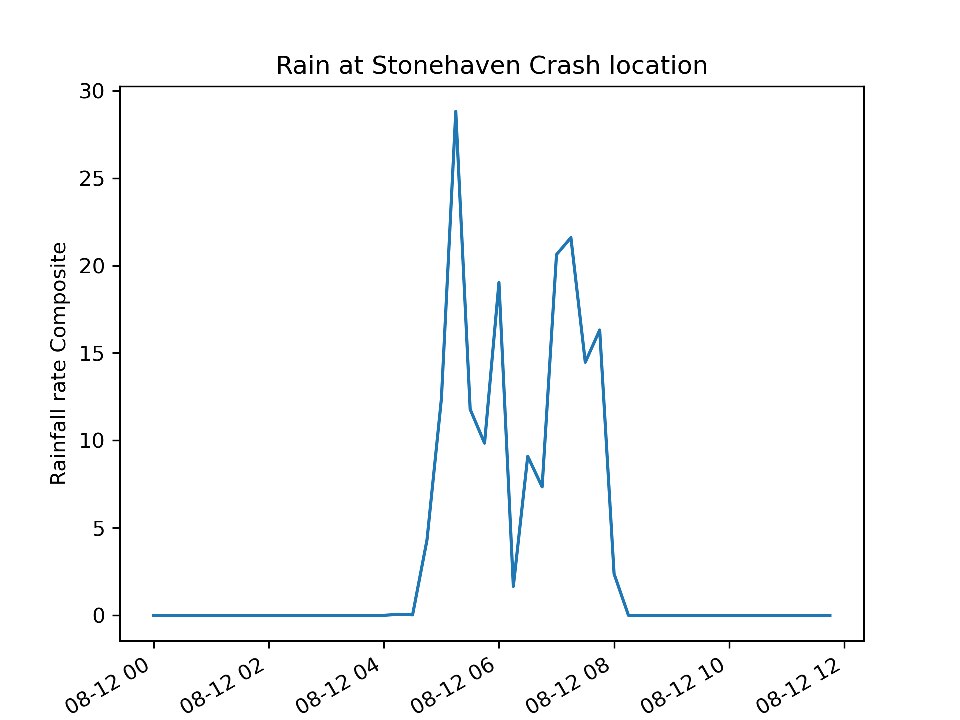
\includegraphics[width=100mm]{stonehavendayraingraph}
    \end{center}
    \caption{A graph of the rainfall at the Stonehaven crash location.
    X-axis is the date and hour (24-hour clock) of the rainfall measurement,
        ranging across the morning of the 12th of August 2020.
    Y-axis is the rainfall measured in mm/h.}
    \label{fig:stonehavendayraingraph}
\end{figure}

From figure~\ref{fig:stonehavendayraingraph},
    the rainfall event begins at 4:15 and ends at 8:15.
The rainfall at the crash location is then given in sixteen 15-minute chunks of time,
    or as across four hours.

This may suggest a four-hour event definition should be used.
However, this was not done for two reasons.
First, it is clear that the rainfall occurred in two 2-hour peaks,
 so a 4-hour definition would not be appropriate for this event.
Second, in section~\ref{subsec:radarprocess},
    the radar data is processed into chunks,
    each of which start on an increment of the length of time of the event.
While this would accurately capture this 4-hour storm, being between 4:00 and 8:00,
    an event from 6:00 to 10:00 would be considered two events of half the size.

A one-hour peak was then used instead.
This was as it allowed storms of a similar length to be quantified by their peak rainfall.

\subsubsection{Rainfall in the Stonehaven region}

\begin{figure}[H]
    \centering

    \begin{subfigure}{0.48\textwidth}
        \centering
        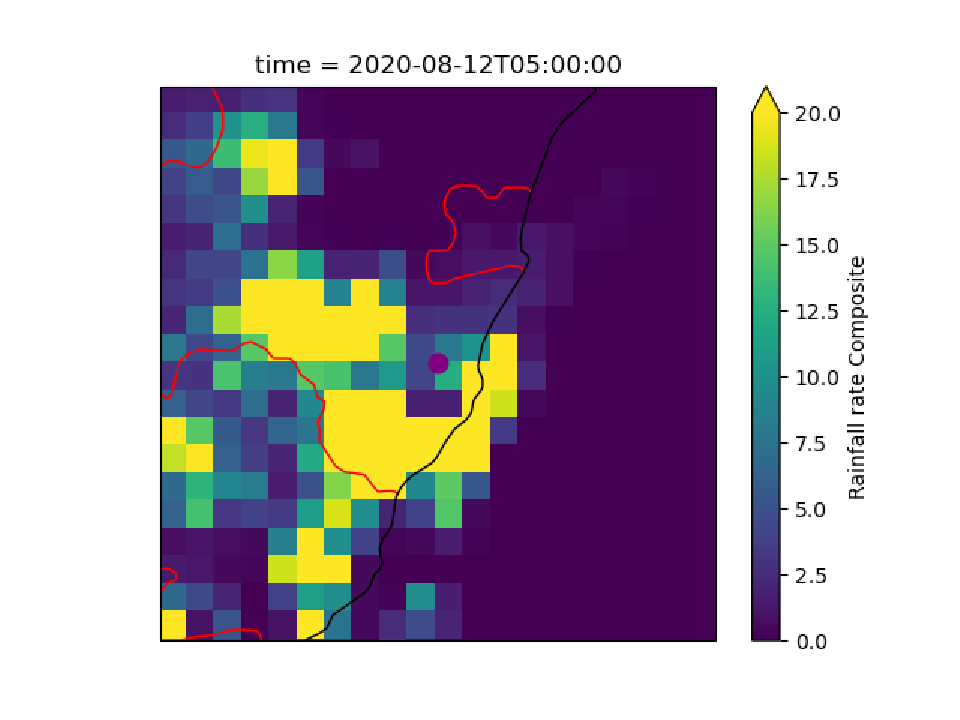
\includegraphics[width=\linewidth]{stonerain5}
    \end{subfigure}
    \hfill
    \begin{subfigure}{0.48\textwidth}
        \centering
        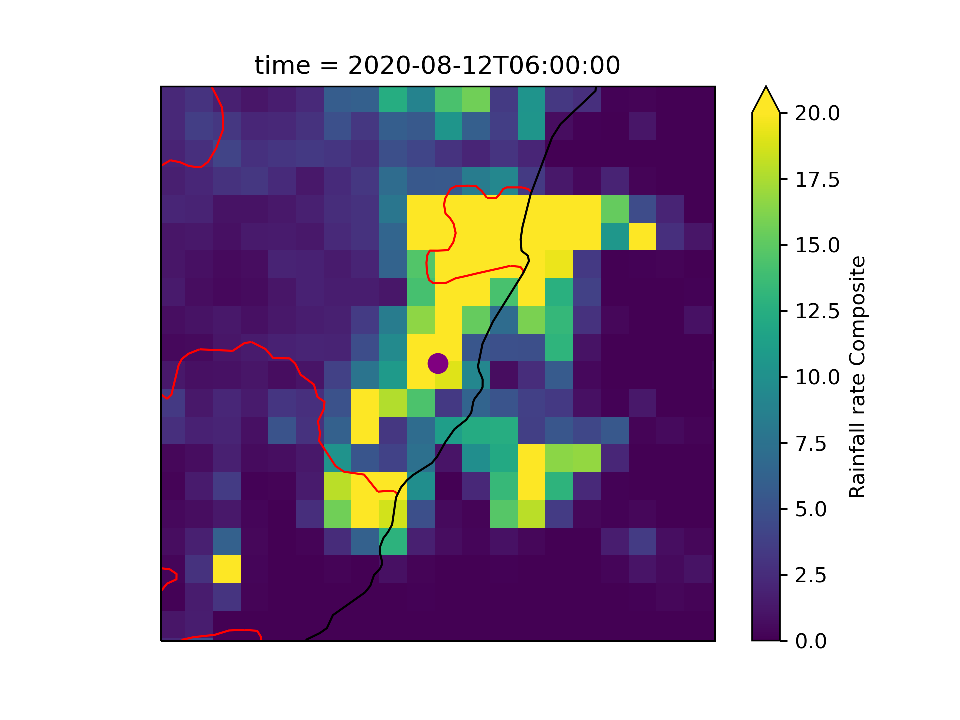
\includegraphics[width=\linewidth]{stonerain6}
    \end{subfigure}

    \vspace{\baselineskip}

    \begin{subfigure}{0.48\textwidth}
        \centering
        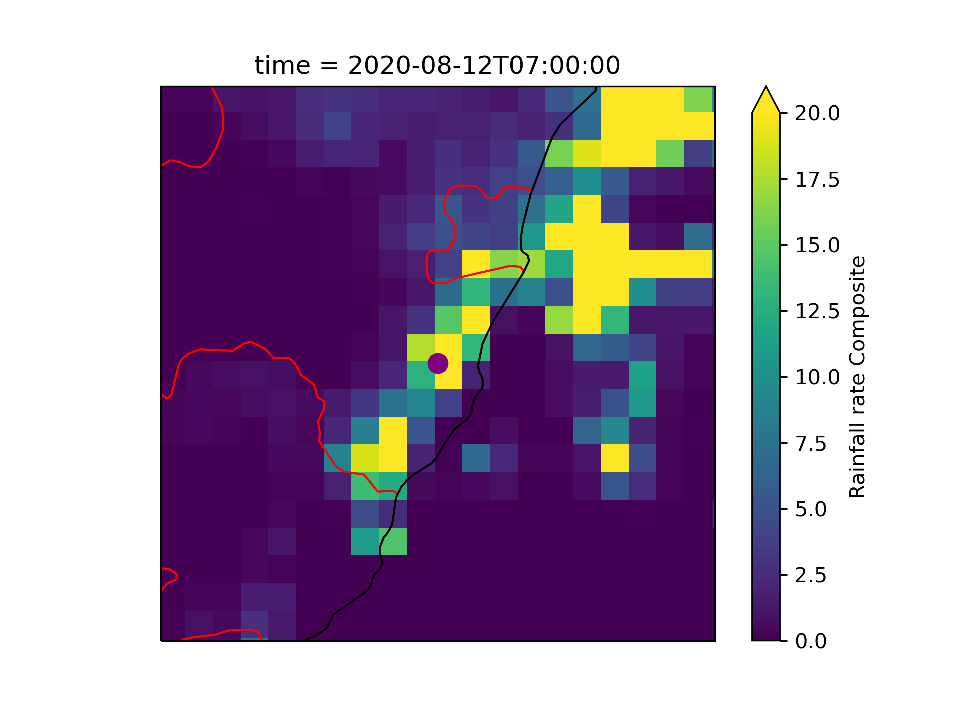
\includegraphics[width=\linewidth]{stonerain7}
    \end{subfigure}
    \hfill
    \begin{subfigure}{0.48\textwidth}
        \centering
        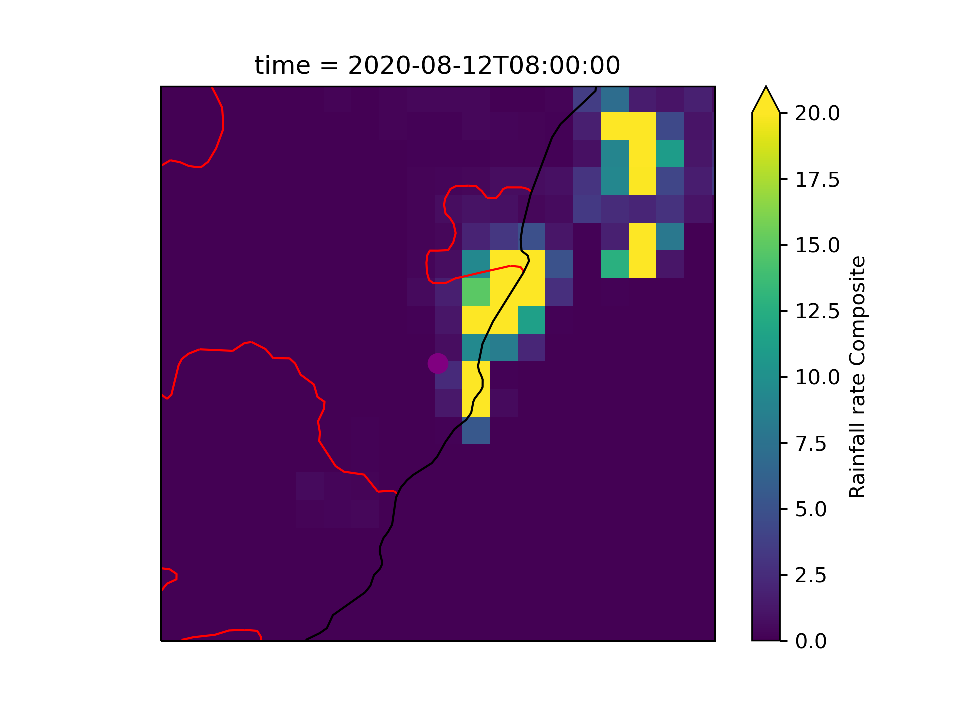
\includegraphics[width=\linewidth]{stonerain8}
    \end{subfigure}
    \caption{Rainfall in the Stonehaven region (+/- 50km of Stonehaven)
        at times of 5, 6, 7 and 8AM of the 12th August 2020,
        in the top left, top right, bottom left and bottom right respectively.
    Scale is mm/h.
    Black lines are coastlines, red lines are local authority boundaries.
    Purple dot is the crash location.}
    \label{fig:stoneregionrain}
\end{figure}

Figure~\ref{fig:stoneregionrain} shows the rainfall in the Stonehaven region,
    demonstrating the movement of the storm North-East throughout the morning of the event.
This figure is also available as an animation using data from 15-minute intervals,
    showing the storm moving as expected.

The figure also suggests that the event covers a large area,
    validating the use of the coarser-resolution 5km dataset as sufficient to describe the event.
One unfortunate consequence of using the 5km dataset is on the rainfall described in figure~\ref{fig:stonehavendayraingraph},
    as the crash location lies near the boundary of four cells, yet the data is only taken from the nearest cell,
    leading to the graph being less accurate approximation of the rainfall at the crash location than would be given by a 1km resolution dataset.

\subsection{Further Constraints}\label{subsec:furthercons}

\subsubsection{Stonehaven Geography}

\begin{figure}[H]
    \centering
    \begin{subfigure}{0.48\textwidth}
        \centering
        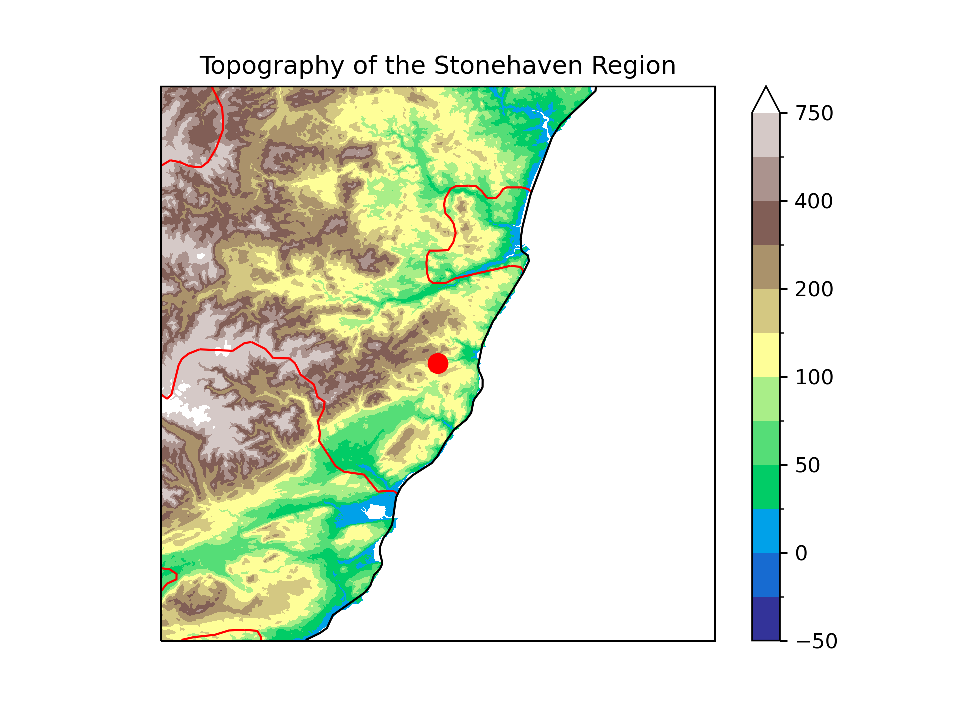
\includegraphics[width=\linewidth]{stonetopog90}
    \end{subfigure}
    \hfill
    \begin{subfigure}{0.48\textwidth}
        \centering
        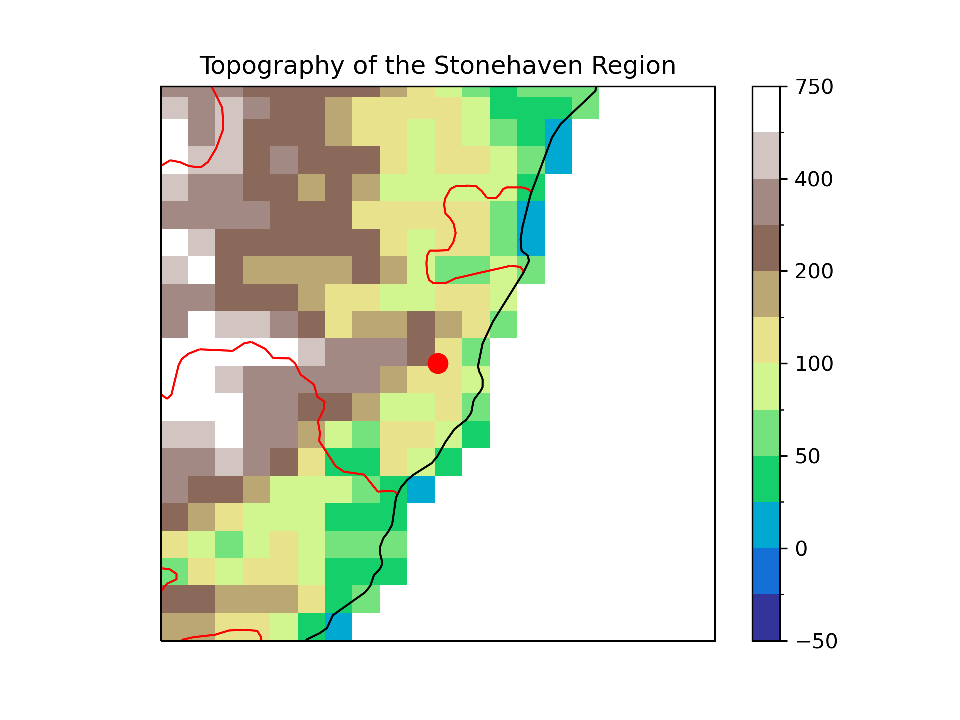
\includegraphics[width=\linewidth]{stonetopog4950}
    \end{subfigure}
    \caption{Plot of the topography in the Stonehaven region.
    Scale is in meters.
    Left is the raw data (at 90mx90m resolution),
    right is the resampled data (at 4950mx4950m resolution) as used for future processing.
    Black lines are coastlines, red lines are local authority boundaries.
    Red dot is the crash location.}
    \label{fig:stonetopog}
\end{figure}

The 4950m resolution data shown in figure~\ref{fig:stonetopog} was found by taking a mean average of 55 of the data points in each dimension,
    giving each grid cell an average of 3250 raw data points.

The area of the Stonehaven crash is around the 200m contour,
    with the crash occurring at around 100m,
    due to the cutting the railway passes through.
Looking at figure 26 of~\cite{RAIB_2022},
    the drain responsible for the crash is 150m above sea level.
Furthermore, the drain's catchment reaches close to 200m.

The topography of the region for the event attribution analysis was then chosen to be from 0m (sea level),
    to 400m.
This is done to make the topography around the crash location typical for the region in which the analysis is performed.
A 200m limit was suggested,
    to match the limit taken in~\cite{Tett_Soon},
    but was not taken forward as this had the potential to give too few data points to define an event.

\begin{figure}[H]
    \begin{center}
        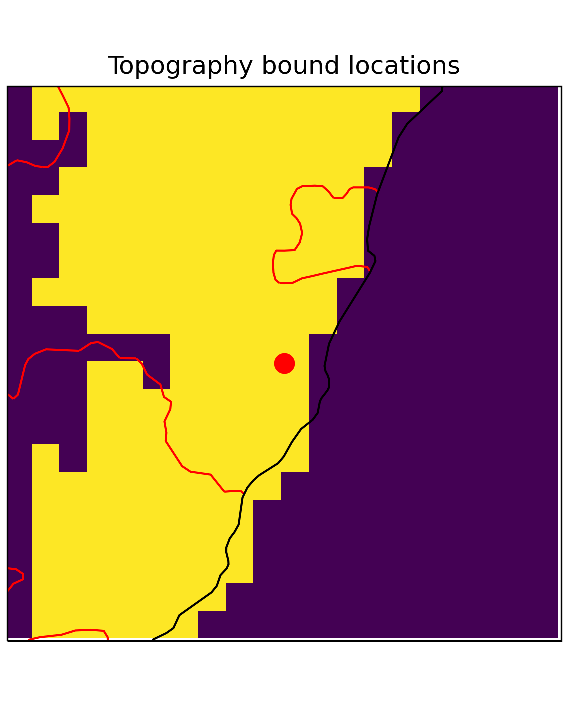
\includegraphics{stonetopogcut}
    \end{center}
    \caption{Map of the Stonehaven region with radar data grid cells (5kmx5km) within a topographical range of 0--400m in yellow,
    grid cells outside of range in violet.
    Black lines are coastlines, red lines are local authority boundaries.
    Red dot is the crash location.}
    \label{fig:stonetopogallowed}
\end{figure}

Out of the 400 grid cells in the Stonehaven Region,
    data is taken from 185 of the grid cells.
This is as 194 of the grid cells are not over land,
    and an additional 21 grid cells have too high topography.

As the radar data is at a 5km resolution,
    while the resampled topography data is at a 4950m resolution,
    the XArray \texttt{interp\_like} method is used to get a linear interpolation for the height at each 5km grid cell.

\subsection{Processing and Fitting the Radar Data}\label{subsec:radarprocess}

The steps used in this section are identical to those used to processing and fitting the radar data for the Edinburgh cloudburst event~\cite{Tett_Soon},
    with changes made to fit the different definition and region in this case.

\subsubsection{Computing Maxima}

As the goal was to use an Extreme Value distribution to model the data,
    it is necessary to draw the extrema out from the data.
The dataset itself~\cite{radar_data} is composed of \texttt{.tar} files, each of which containing the radar data of a given day.

The \texttt{process\_radar\_data} Python script finds the maximum one-hour rainfall in each of these daily datasets and
    uses these to generate a dataset with the one-hour maximum rainfall and the time of the one-hour maximum rainfall
    at all points in the Stonehaven Region for a given month, in a NetCDF format
The \texttt{combine\_summary} Python script then takes these monthly maxima and their times and combines them into a single dataset,
    again as a NetCDF .

These Python scripts are called by the Shell scripts \texttt{run\_jobs} and \texttt{run\_combine} respectively.
The Shell scripts are run on a JASMIN Science Analysis Server and submit the Python scripts as SLURM jobs to the LOTUS Batch Processing Cluster,
    allowing all the monthly maxima to be computed in a single script and the combination of the datasets to access an amount of memory to make the task feasible.

The \texttt{get\_radar\_data} function in the \texttt{stonehavenRainLib} Python script then selects the summer months and
    combines them to get the maximum hourly rainfall in the summer of each year,
    along with the time of the maxima.
This function also applies the topographical height mask described in subsection~\ref{subsec:furthercons},
    returning an XArray DataSet of the radar data that will be used to describe and generate statistics for the event.

\subsubsection{Computing Events and Definition}

Now that the seasonal maxima have been found,
    the data can be used to define events.
This process is done in the \texttt{gen\_radar\_data} function in the \texttt{stonehavenRainLib} Python script.
The seasonal maxima,
    of which there is one for each grid cell in each year in the dataset,
    are grouped by the time in which they occurred.

These groups are 12-hour periods,
    representing either the AM or PM hours of a day.
Each group is then an event,
    containing the grid cells which experienced their maximum hourly rainfall within the group's time period.
The groups with less than 10 grid cells were discarded,
    as these events are less than 250km$^2$ in size and
    so do not represent events similar enough to the Stonehaven event.

This gives a final event definition as 250km$^2$ of the land below 400m and within +/- 50km of Stonehaven
    experiencing their annual summer hourly rainfall maxima in the same 12-hour period.

For each event, the 0.05, 0.1, 0.2, 0.5, 0.8, 0.9 and 0.95 quantiles were found and returned in a dataset.
The magnitude of a given event is defined by its 0.95 quantile.

\begin{figure}[H]
    \centering
    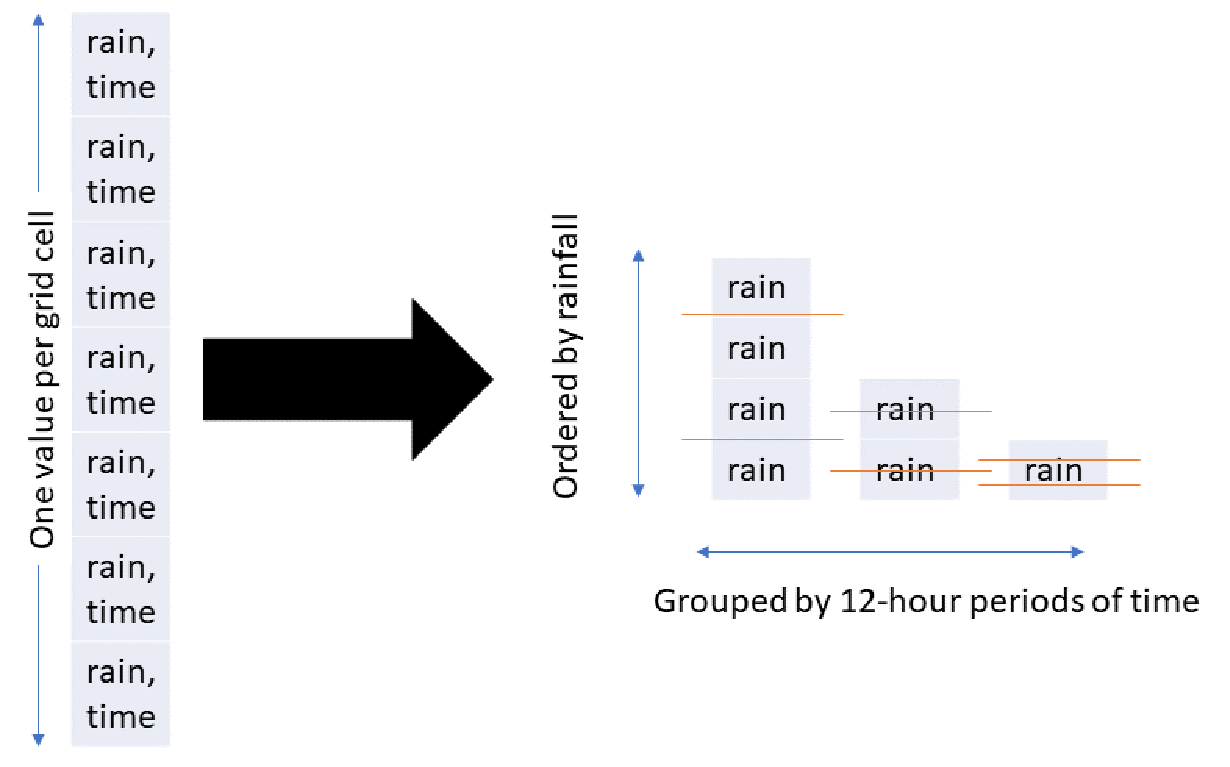
\includegraphics[width=80mm]{dataprocessschematic}
    \caption{Diagram representing the data processing after the maxima of each grid square has been found,
    within each year.
    `rain' represents the summer maximum rainfall in a grid cell,
        `time' represents the time of this maximum,
        red horizontal lines represent the taking of quantiles from the rainfall maxima.
    Number of data points and quantiles are not to scale.}
    \label{fig:dataprocessschematic}
\end{figure}

\subsubsection{Fitting event distribution}

The radar data is fit to a GEV distribution with the \texttt{comp\_radar\_fits} Python script,
    which calls the \texttt{gev\_r} Python library to run code in R .
The `fevd', fit extreme value distribution,
    command in R is used to fit an extreme value distribution to the radar data,
    which uses MLE, as described in subsection~\ref{subsec:parameterest}.
This command is applied each of the quantiles of the event,
    with the events as the data points,
    giving the parameters of GEV distributions describing each quantile of the events.
With these parameters generated,
     it was possible to find the empirical return period for the Stonehaven event.

To generate uncertainties,
    a Monte Carlo bootstrap method is used,
    given in the \texttt{mc\_dist} function.
This involved generating a list of the same size of the number of events,
    taking a random sample with replacement,
    then applying the `fevd' command to each sample.

1000 samples were taken,
    of which 9 provided anomalous (negative) location or scale parameters,
    and so were discarded.
The discarding process was valid as the value of these parameters was ~-100,
    while all other samples had values of these parameters between 2 and 15,
    as well as that removing this few samples would not have a significant effect on the 95\% confidence interval.
The 991 samples left are greater than the 800 suggested by Booth and Sarkar~\cite{Booth_Sarkar_1998}
    for an effective error estimation.

\section{Modelled Data}\label{sec:model}

The model data used in this section is
    the Met Office Hadley Centre's UKCP18 Convection-Permitting Model Projections for the UK at 2.2km resolution~\cite{model_data}.
This dataset was chosen as the resolution is less than 5km,
    and so is able to accurately represent convective storms.

The CPM ensemble consists of 12 members and covers the 100 years from 1981 to 2080,
    modelling the RCP8.5 emissions scenario.
In this investigation,
    the model's hourly temperature and rainfall data will be used

\subsection{Pre-processing}\label{subsec:preprocess}

The CPM data used is on longitude-latitude coordinates,
    with a north pole rotated to near the region the model covers.
The location of the Stonehaven crash in this alternative coordinate system was found using the \texttt{comp\_rotated\_coords} Python script,
    using CartoPy for the computations.
This coordinate rotation was also done for the four weather stations used to compute Central England Temperature (CET).

The pre-processing of the CPM data is done using the \texttt{ens\_seas\_max\_coarsen} python script,
    which finds the seasonal one-hour rainfall maxima for each grid cell.

\subsubsection{Coarsening}

The CPM data uses a 2.2km resolution,
    while the radar data uses a 5km resolution.
To account for this,
    the radar data is coarsened using the XArray \texttt{.coarsen} and \texttt{.mean} methods,
    taking the mean average of four 2.2kmx2.2km grid cells, giving 4.4kmx4.4km grid cells.

The height mask for the CPM was in the same 2.2km resolution
    and so required the same pre-processing

\subsubsection{Height mask}

To match the event definition in section~\ref{subsec:radarprocess},
    a similar height mask must be used,
    with the same limits of 0m to 400m.

\subsection{Covariates}\label{subsec:covfit}

\subsubsection{Time Series}

The \texttt{comp\_cpm\_ts} Python script was used to compute the time series.
This script takes each month in each ensemble member the CPM data and computes 3 values.
These are computed using the 2.2km data without the coarsening or height mask.
First is the Central England Temperature,
    which takes the CPM data's average monthly temperature at the weather stations used to define CET,
    while the other two time series use the average monthly temperature and precipitation in the Stonehaven Region.

Two additional monthly time series were computed in the \texttt{analyse\_cpm\_data\_rolling} Python script.
One of these takes the median extreme precipitation across the Stonehaven Region
    using the extrema processed in \texttt{ens\_seas\_max\_coarsen.sh},
While another uses the temperature in the Stonehaven Region to find the Saturation Specific Humidity.

The formula used for this is the August-Roche-Magnus approximation to the Clausius-Clapeyron relation~\cite{Alduchov_Eskridge_1996}, given by:
\begin{equation}\label{eq:qsat}
    e_s = 6.112 \exp\left( \frac{17.6 T}{T + 243.5} \right)
\end{equation}
Where $T$ is the temperature in degrees Celsius.

Each time series had 14400 members,
    with 12 ensemble members providing data for the 1200 months across the 100-year window of the model.

\subsubsection{Fitting Covariates}

In a method analogous to the \texttt{comp\_radar\_fits} Python script calling the \texttt{gev\_r} library to use R to fit
    a distribution to the radar rainfall extrema in subsection~\ref{subsec:radarprocess},
    \texttt{analyse\_cpm\_data\_rolling} calls the \texttt{gev\_r} library to perform fits on the model rainfall extrema.
This is done with the same `fevd' command in the extRemes R library~\cite{extremes_R},
    except done with the time series as covariates.

For this,
    the location and scale parameters are allowed to change linearly with the variable $x$.
The parameters are then $\mu = \mu_0 + x\mu_1$ and $\sigma = \sigma_0 + x\sigma_1$.
The analysis is then repeated with the shape parameter also allowed to vary in the form $\xi = \xi_0 + x\xi_1$.

\subsection{Calculating Risk Ratios}\label{subsec:riskratios}

\chapter{Results and Analysis}\label{ch:results}

\section{Results}\label{sec:results}

\begin{comment}
This section should detail the obtained results in a clear,
easy-to-follow manner. It is important to make clear what are original
results and what are repeats of previous calculations or computations.
Remember that long tables of numbers are just as boring to read as
they are to type-in!

Use graphs to present your results wherever practicable.

Results or computations should be presented with uncertainties
(errors), both statistical and systematic where applicable.

Be selective in what you include: half a dozen \emph{e.g.}~tables that
contain wrong data you collected while you forgot to switch on the
computer are not relevant and may mask the correct results.
\end{comment}

\subsection{Radar Data Fit}\label{subsec:radardatafit}

%  TODO insert return chart

\subsection{Model Correlations}\label{subsec:modelcorr}

%  TODO insert CET scatter

\subsection{Risk Ratios}\label{subsec:riskratio}

%  TODO insert prob_radar_CPM

%  TODO insert plot showing overlap of distributions w/ parameters

\section{Discussion}\label{sec:discussion}

\begin{comment}
This section should give a picture of what you have taken out of your
project and how you can put it into context.

This section should summarise the results obtained, detail conclusions
reached, suggest future work, and changes that you would make if you
repeated the project.
\end{comment}

\subsection{Event Definition}\label{subsec:diseventdef}

%  TODO mention lack of trend analysis due to lack of radar data

%  TODO mention Koppen in analysis

\subsection{Model Resolution}\label{subsec:dismodeldef}

Mention~\cite{Kendon_Fischer_Short_2023}
%  TODO insert chart w various coarsenings

\subsection{Model Validity}\label{subsec:dismodelvalid}

\chapter{Conclusions}\label{ch:conclusions}

\begin{comment}
This is the place to put your conclusions about your work. You can
split it into different sections if appropriate. You may want to include
a section of future work which could be carried out to continue your
research.

The conclusion section should be at least one page long, preferably 2
pages, but not much longer.
\end{comment}

\appendix
% the appendix command just changes heading styles for appendices.

%  TODO insert code behind each figure

\chapter{Stuff that's too detailed}

Appendices should contain all the material which is considered too
detailed to be included in the main body of the text, but which is
important enough to be included in the thesis.

Perhaps this is a good place to mention \BibTeX.

You can do references in the simple way explained in the introduction,
or you can use \BibTeX.


\bibliographystyle{unsrt}
\bibliography{ref}




\end{document}

